
\section{Experiments}
\label{sec:evaluation}

We evaluate PGR against multiple retrieval and reasoning baselines on long-term, multi-session conversational tasks to test whether prospective, simulation-driven retrieval provides more anticipatory and contextually grounded personalization than conventional retrospective retrieval. We use three benchmarks. The \textbf{MemoryQuest} benchmark (Section~\ref{sec:dataset}) includes 50 users and \textbf{535 queries} across 20 task domains; each query requires \textbf{3--5} references, which serve as retrieval and answer ground truth. Users have an average of \textbf{77.6 sessions} with \textbf{6.2 exchanges per session}. {ImplexConv}~\cite{li2025implexconv} provides long multi-session dialogues with opposed and supportive implicit-reasoning scenarios; we use only the \textit{opposed} setting, where relevant context is semantically distant and contradicts the surface persona. Each query has a single required reference; we evaluate \textbf{196 queries} across 85 users (sampled from 1,550 users in the full dataset), with an average of \textbf{110 sessions} and \textbf{5.8 exchanges per session}. {PersonaMem}~\cite{jiang2025personamem} provides persona profiles and long conversation histories; we use the 32k chat-history variant and sample \textbf{50 random profiles}, excluding \texttt{ask\_to\_forget} and \texttt{sensitive\_info} queries to focus on preference-grounded personalization, yielding \textbf{894 queries} (sampled from 200 users and 3,441 queries in the full dataset); each user has a single long chat history averaging \textbf{116 exchanges} ($\sim$32k tokens). Overall, we evaluate 1,625 queries across 185 user profiles. We release the MemoryQuest generation framework to support reproducibility and scaling to 1,500+ user profiles.


\subsection{Baselines}
We compare PGR against three other state of the art memory retrieval baselines. Experiments are run using Azure OpenAI GPT-4o for simulation and answer generation, and \texttt{text-embedding-3-small} for embedding and retrieval \cite{openai2024embeddings}. Additional experiments using PGR-TOT with DeepSeek-V3.2 as the generation model are reported in Appendix~\ref{sec:deepseek_results}.

% \textbf{RAG over Facts.} Standard RAG~\cite{lewis2020rag} retrieves the top-$K$ memory facts most similar to the query by dense embedding similarity ($\tau = 0.3$), appends them as context, and generates a response. We evaluate at $K = 20$.

% \textbf{RAG over Chats.} A variant of RAG that retrieves chunks of raw conversation sessions rather than structured facts, using the same embedding similarity. This tests whether using conversational context directly is preferable to distilled facts. We evaluate at $K = 5$ chunks.

\textbf{Mem0$^\texttt{g}$.} \cite{chhikara2025mem0} utilizes a Neo4j-backed entity-relation graph to store memories. Retrieval combines vector search with graph relation extraction to test if explicit relational structures can compensate for the absence of prospection. We evaluate at $K=20$.

\textbf{GraphRAG.} \cite{edge2024graphrag} indexes dialogue sessions into an entity graph and retrieves the top-$K=5$ community reports via embedding similarity to evaluate structured graph summarization as a non-prospective alternative.

\textbf{TaciTree.} \cite{li2025implexconv} utilizes a hierarchical tree for implicit reasoning retrieval. Facts are clustered via UMAP and Gaussian Mixture Models (max size $k=6$), then summarized by an LLM to form leaf nodes. The tree is built iteratively until the root contains $L=15$ clusters. At inference, an LLM performs top-down pruning to select the top-$K=5$ most relevant leaf summaries, avoiding exhaustive search.

\paragraph{Hyperparameters.} For all PGR variants, we set the convergence threshold to $\delta = 5$ newly retrieved facts and the maximum number of refinement iterations to $I_{\max} = 10$. Query-only baselines retrieve the top $K = 20$ facts; each PGR sub-query retrieves the top $K = 5$ facts with embedding similarity threshold $\tau = 0.3$. For query augmentation in Phase 2, we apply a stricter threshold $\tau_o = 0.6$ to ensure only high-confidence context informs refinement. These settings are fixed across all datasets.


\subsection{Evaluation Metrics}

We use Azure OpenAI GPT 5.2 for evaluating the responses. Prompts are provided in the Appendix. 

\begin{wrapfigure}{r}{0.44\textwidth} % {r} for right side, 0.45 for just under half width
    \centering
    \vspace{-10pt} % Adjust to align top with text
    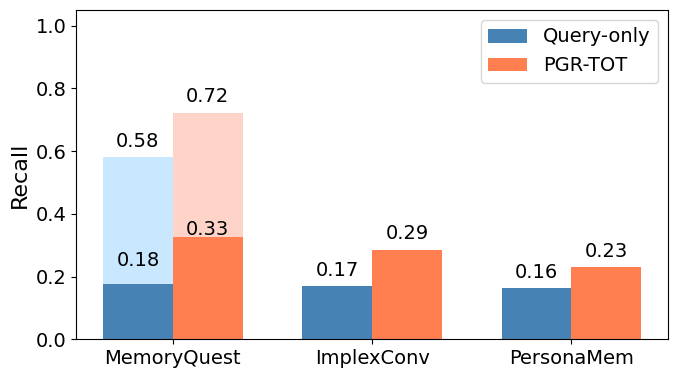
\includegraphics[width=0.42\textwidth]{figures/rag-vs-pgr.png}
    \caption{\small{Results comparing Retrieval Recall using Query-only and PGR-TOT. For MemoryQuest, lighter bars: Recall, and darker bars: Recall$_{Exact}$.}}
    \label{fig:rag-vs-pgr}
    \vspace{-12pt} % Adjust to reduce space below caption
\end{wrapfigure}

\paragraph{Retrieval-level:}
For each method, we obtain the \emph{retrieved context} (e.g., the set of facts or chat excerpts retrieved to generate the answer). The LLM is given the query, the list of required references, and the retrieved context, with a simple instruction to independently identify (binary, Yes/No) whether each reference is found explicitly or implicitly. We report \textbf{Recall} as the fraction of required references judged present, averaged over queries. For ImplexConv and PersonaMem, the judgment is binary. Since MemoryQuest has multiple references, we report the fraction as well as \textbf{Recall$_{Exact}$}, which is 1 if all references are identified, else 0.

\paragraph{Response-level:}
We also compare the \emph{final answers} generated using PGR and each baseline by constructing an LLM-based user simulator that has knowledge of all facts about the user context. For each query, the two responses are presented to the simulated user, along with the list of required references. The output indicates which response is more useful and proactive (acknowledging past context, anticipating needs, and giving actionable guidance) or marks a tie. We repeat this experiment twice for each query by reversing the order of responses to avoid position bias and take the average of both. Prompts are provided in the Appendix. We report \textbf{Win Rate} (\%) of PGR versus each baseline as the fraction of queries where the simulated user prefers the PGR response. We also conducted a human study to evaluate the efficacy of LLM-as-a-Judge on a smaller subset of queries, comprising approximately 4\% of MemoryQuest, 5\% of ImplexConv, and 2\% of PersonaMem queries. Human evaluations were conducted on each PGR-baseline pair, and results are reported in Table \ref{tab:main_results}. Experiments were conducted on Amazon MTurk. IRB exemption was received for this study.



\section{Results and Discussion}
\label{sec:results}


\begin{table}[t]
\centering
\setlength{\tabcolsep}{4pt}
\caption{Average Recall and Win Rate(\%) of PGR-TOT over baseline methods evaluated on MemoryQuest, ImplexConv, and PersonaMem datasets. Human* evaluations were done on a subset of queries. Higher is better.}
\vspace{1pt}
\begin{tabular}{l|ccccc|ccc|ccc}
\toprule
\textbf{Dataset $\rightarrow$} & \multicolumn{5}{c|}{\textbf{MemoryQuest}} 
& \multicolumn{3}{c|}{\textbf{ImplexConv}} 
& \multicolumn{3}{c}{\textbf{PersonaMem}} \\
\cmidrule(lr){2-6} \cmidrule(lr){7-9} \cmidrule(lr){10-12}
\textbf{Method $\downarrow$} & Recall & Recall$_{Exact}$ & \multicolumn{2}{c}{Win Rate$_{PGR}$} & & Recall & \multicolumn{2}{c}{Win Rate$_{PGR}$} & Recall & \multicolumn{2}{c}{Win Rate$_{PGR}$} \\
\cmidrule(lr){4-5} \cmidrule(lr){8-9} \cmidrule(lr){11-12}
& & & \small LLM & \small Humans$^*$ & & & \small LLM & \small Humans$^*$ & & \small LLM & \small Humans$^*$ \\
\midrule
GraphRAG & \med{0.160} & \low{0.003} & \vhigh{96.6} & \high{90.0} & & \low{0.072} & \vhigh{96.2} & \high{70.0} & \low{0.011} & \vhigh{98.4} & \high{80.0} \\
TaciTree & \med{0.235} & \low{0.024} & \vhigh{94.3} & \high{75.0} & & \low{0.122} & \high{89.9} & \med{60.0} & \low{0.073} & \high{88.7} & \med{65.0} \\
Mem0$^{\texttt{g}}$ & \med{0.256} & \low{0.015} & \vhigh{94.7} & \vhigh{95.0} & & \low{0.050} & \vhigh{93.5} & \med{70.0} & \low{0.121} & \vhigh{92.9} & \med{65.0} \\
\textbf{PGR-TOT} & \vhigh{\textbf{0.723}} & \high{\textbf{0.326}} & - & - & & \med{\textbf{0.286}} & - & - & \med{\textbf{0.229}} & - & - \\
\bottomrule
\end{tabular}
\label{tab:main_results}
\end{table}

Results in Table~\ref{tab:main_results}, demonstrate that Prospection-Guided Retrieval (PGR) outperforms traditional retrieval baselines across all evaluated datasets and metrics.

\paragraph{Higher Retrieval Recall.} 
On the MemoryQuest benchmark, PGR-TOT achieves a recall of \textbf{0.723}, nearly tripling the performance of the strongest baseline, Mem0 (0.256), and vastly exceeding GraphRAG (0.160). This trend persists across ImplexConv and PersonaMem, where PGR consistently surfaces relevant context that passive semantic search fails to identify. These gains are particularly pronounced in \textbf{Recall$_{Exact}$} metrics (\textbf{0.326} vs.\ 0.015 for Mem0), indicating that PGR is uniquely capable of retrieving the complete "thread" of facts required for complex reasoning.


Figure \ref{fig:rag-vs-pgr} compares retrieval performance between a standard \textit{Query-only} baseline and PGR-TOT. We decompose these results into Recall$_{Exact}$ (dark regions)—representing queries where the entire ground-truth set is recovered—and fractional recall (light regions). 


The visualization underscores the "prospection gap": while the Query-only baseline struggles with a total recall of only \textbf{0.58} on MemoryQuest, PGR-TOT achieves \textbf{0.723}.  This demonstrates that by simulating future trajectories, PGR effectively bypasses the semantic similarity bottleneck, successfully reconstructing the complete "thread" of chronologically distant facts required for complex personalization.


\begin{wraptable}{r}{0.45\textwidth}
\centering
\renewcommand{\arraystretch}{1.2}
\setlength{\tabcolsep}{4pt} % Slightly reduced for wrapping
\vspace{-12pt}
\caption{Aggregated comparison matrix between judgments of humans (rows) and LLM (columns).}
\small
\begin{tabular}{l|>{\centering\arraybackslash}p{1.1cm}>{\centering\arraybackslash}p{1.1cm}>{\centering\arraybackslash}p{1.1cm}}
\toprule
\textbf{Human $\backslash$ LLM} & \textbf{PGR} & \textbf{Tie} & \textbf{Baseline} \\
\midrule
\textbf{PGR} & \cellcolor{pink!70} 70.0 & \cellcolor{pink!20} 4.0 & \cellcolor{pink!0} 2.0 \\
\textbf{Tie} & \cellcolor{pink!20} 8.0 & \cellcolor{pink!0} 0.0 & \cellcolor{pink!10} 0.7 \\
\textbf{Baseline} & \cellcolor{pink!40} 12.0 & \cellcolor{pink!20} 2.0 & \cellcolor{pink!20} 1.3 \\
\bottomrule
\end{tabular}
\label{tab:human-llm-matrix}
\vspace{-0pt}
\end{wraptable}


\paragraph{High-Quality Response Generation.} 
The improvement in retrieval translates directly to superior response quality. As shown in Table~\ref{tab:main_results}, PGR achieves dominant win rates in LLM-as-a-judge evaluations, ranging from \textbf{88.7\% to 98.4\%}. Crucially, human evaluations confirm this preference, with annotators favoring PGR responses in \textbf{60--95\%} of cases. Table~\ref{tab:human-llm-matrix} reports the aggregated human-vs-LLM agreement matrix across all baseline pairs and datasets; humans and the LLM judge agree on preferring PGR in \textbf{70\%} of all evaluated cases. Human annotators noted that PGR-based responses were significantly more proactive, correctly utilizing long-term personal history to provide actionable guidance. 


The empirical success of PGR highlights a structural limitation in contemporary ``lookup-based'' memory architectures. By decoupling memory retrieval from underlying storage and implementing an iterative \textit{simulate $\rightarrow$ retrieve $\rightarrow$ refine} cycle, PGR enables the system to proactively anticipate informational needs. 
%
\begin{wraptable}{r}{0.45\textwidth}
    \centering
    \setlength{\tabcolsep}{4pt}
    \vspace{-.5em} 
    \caption{Effect of prospection strategies.}
    \small
    \begin{tabular}{l|cc}
        \toprule
        \textbf{PGR Method} & \textbf{Recall} & \textbf{Win Rate (\%)} \\
        \midrule
        TOT \textit{vs} COT  & \high{0.723 \textit{\textbf{>}} 0.718} & \low{55.67} \\
        \bottomrule
    \end{tabular}
    \label{tab:ablation-tot-cot}
    \vspace{-1em}
\end{wraptable}
%
This mechanism facilitates the identification of ``latent'' memories: contextual facts that, while lacking immediate semantic proximity to the current dialogue turn, are crucial for achieving the user's long-term objectives. Our findings suggest that \textit{prospection} is a key paradigm for developing highly personalized, context-aware conversational agents.

\begin{table}[h]
    \centering
    \setlength{\tabcolsep}{3pt} % Slightly reduced padding to ensure fit
    
    % First Table (Left)
    \begin{minipage}{0.49\textwidth}
        \centering
        \caption{Effect of iterative prospection.}
        \begin{tabular}{l|cc|c}
            \toprule
            \textbf{Method} & \multicolumn{2}{c}{\textbf{Recall}} & \textbf{Win Rate} \\
             & \textbf{Base} & \textbf{Iterative} & \textbf{Iterative} \\
            \midrule
            PGR-TOT & \med{0.677} & \high{0.723} & \high{70.13} \\
            PGR-COT & \med{0.645} & \high{0.718} & \high{75.41} \\
            \bottomrule
        \end{tabular}
        \label{tab:ablation-iterative}
    \end{minipage}
    % Second Table (Right)
    \begin{minipage}{0.49\textwidth}
        \centering
        \caption{Effect of prospection summary.}
        \begin{tabular}{l|cc|c}
            \toprule
            \textbf{Method} & \multicolumn{2}{c}{\textbf{Recall}} & \textbf{Win Rate} \\
             & \textbf{$\sim$PAG} & \textbf{PAG} & \textbf{PAG} \\
            \midrule
            PGR-TOT & \med{0.703} & \high{0.722} &  \high{75.73} \\
            PGR-COT & \high{0.722} & \high{0.735} &  \high{74.37} \\
            \bottomrule
        \end{tabular}
        \label{tab:ablation-prospection}
    \end{minipage}
\end{table}


We conduct ablations on MemoryQuest to isolate the contributions of iterative retrieval, the use of the prospection summary in answer generation, and the type of prospection strategy within PGR.

\textbf{Iterative Prospection} consistently improves memory recall and answer quality. As shown in Table~\ref{tab:ablation-iterative}, both PGR-COT and PGR-TOT achieve higher recall and win rates when sub-queries are retrieved and refined iteratively.

\textbf{Prospection-Augmented Generation (PAG).} Conditioning answer generation on the prospection summary further boosts performance. Table~\ref{tab:ablation-prospection} shows that including PAG improves recall and win rate over using retrieved facts alone for both COT and TOT variants.

\textbf{Prospection Strategy.} Comparing PGR-TOT and PGR-COT (Table~\ref{tab:ablation-tot-cot}) reveals that branching tree-of-thought exploration slightly outperforms linear chain-of-thought in Recall, though win rate differences are modest. 

Overall, the results indicate that iterative retrieval, prospection-guided generation, and the choice of prospection strategy each contribute to more effective memory retrieval and response generation in PGR.


\textbf{Limitations.}
PGR’s iterative process improves accuracy by carefully planning and exploring potential future trajectories, but this comes at the cost of additional LLM calls compared to single-pass retrieval. While PGR remains cheaper than TaciTree per query (Appendix Table~\ref{tab:llm-budget}), the multi-phase prospection can be resource-intensive for real-time applications. Future work could reduce this overhead by training specialized lightweight retrievers on the generated prospection traces, enabling faster memory selection while retaining much of the anticipatory reasoning benefit. 
